% File: Harddrive.tex
% Author: Adam Leeper
%------------------------------------------------------------------------------
\providecommand{\isolatedBuild}[1]{#1}% Fallback definition to build normally.
\isolatedBuild{
  \documentclass[11pt,letterpaper]{book}
  %\documentclass[11pt,letterpaper]{book}

% aleeper: I think these are needed for Paul's macros?
\usepackage{epsfig}
\usepackage{epstopdf}

%\makeatletter
%\typeout{The import path is \import@path}
%\makeatother

\usepackage{import}

\subimport{./}{packagesMitiguy.sty}
\subimport{./}{macrosMitiguy.tex}
\subimport{./}{PageStylesMitiguy.tex}
\subimport{./}{macrosLeeper.tex}
   % Found via TEXINPUTS environment variable.
  \isolatedBuildHeader{Rotational Kinematics}
                      {Mechanical Disk Drive Kinematics}
}
%%%
%%%
%%%
\begin{minipage}{0.5\textwidth}
  A computer hard-drive platter \basis{B} spins in an enclosure \basis{N}.
  For convenience, we define unit vectors \uvecxyz{b} fixed in \basis{B}
  with \uvecz{b} perpendicular to the platter. Let point $B_o$ be the center
  of the platter.
  %Note that the exact orientation of \uvecx{b} and \uvecy{b} is irrelevant
  %for this question.
  %
  \\[0.5pc]
  The angular velocity of \basis{B} in \basis{N} is
  $\angvel{B}{N} \equals[\;] \omega_z ~\uvecz{b}$, where $\omega_z$ may
  vary with time.
\end{minipage}
\hfill
\begin{minipage}{0.35\textwidth}
  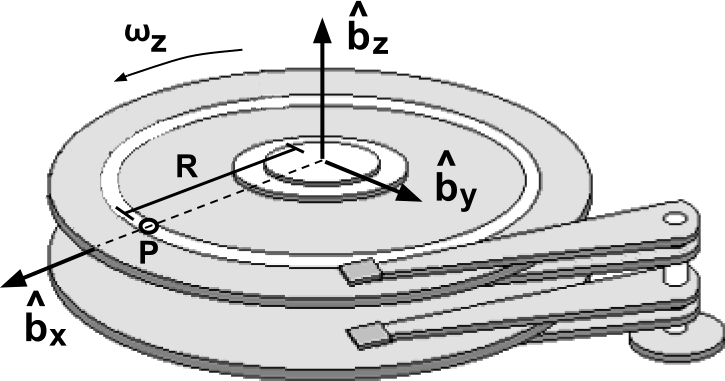
\includegraphics[width=\textwidth]{harddrive_annotated.png}
\end{minipage}
%
%The hard drive organizes data on the platter as concentric circles
%called “tracks,”
%and along each track are individual magnetic regions we will call “bits.”
%Assume bits are small enough to be modeled as points on the platter.
%
\begin{enumerate}
  \item Consider an arbitrary point $P$ on the platter, at a constant
    distance $R$ in the \uvecx{b} direction from the center point $B_o$.
    Derive an expression for $\vel{P}{N}$ in terms of $R$ and $\omega_z$.
    \\[20.0pc]
    %
  \item Hence, use the \textbf{definition} of \textbf{speed} to express
    $P$'s speed in \basis{N}.
    \\[0.0pc]
    Will this speed be the same for all points that lie on the circle of
    radius $R$ from $B_o$?
    \\[15.0pc]
    %
  \clearpage
  \item A typical hard drive has outer radius 1.75", inner radius 0.75",
    and spins at 7200 RPM (revolutions per minute).
    Use your result from (b) to determine how much faster a point on the
    outermost track of the hard drive travels compared to a point on the
    innermost track. Express the result as a \textbf{percentage}.
    \\[18.0pc]
    %
%  \item A hard drive writes data by filling each circular track starting
%    from the outside and working inward. Using your results above or your
%    intuition:
%    \TrueFalse{0} A hard drive can write new data faster (more bits/second)
%    when it is brand new than when the first half of the disk is full.
%    \\[0.0pc]
%  \item Given that a hard drive writes data from outside to inside, and
%    assuming a uniform linear density of bits on each track of the platter,
%    what is the ratio of read and write speed
     %
  \item The hard drive is spinning at 7200 RPM when it is powered down.
    Friction in the device causes the disk to slow down at a
    \textbf{constant} angular acceleration of
    $-200\frac{\mathrm{rad}}{\mathrm{sec}^2}$.
    \textbf{Note:} Pay attention to unit conversions.
    \begin{enumerate}
      \item How many seconds does it take the disk to come to a complete stop?
        %\\[10.0pc]
      \item How many revolutions does the disk make during this interval?
        \\[20.0pc]
    \end{enumerate}
\end{enumerate}
%
\isolatedBuildFooter
